%%%%%%%%%%%%%%%%%%%%%%%%%%%%%%%%%%%%%%%%%%%%%%%%%%%%%%%%%%%%%%%%%%%%%%%%%%%%%%%%%%
\begin{frame}[fragile]\frametitle{}
\begin{center}
{\Large Dataframes in Pandas}
\end{center}
\end{frame}

%%%%%%%%%%%%%%%%%%%%%%%%%%%%%%%%%%%%%%%%%%%%%%%%%%%%%%%%%%
\begin{frame}
  \begin{center}
    {\Large Introduction to Pandas}
  \end{center}
\end{frame}

%%%%%%%%%%%%%%%%%%%%%%%%%%%%%%%%%%%%%%%%%%%%%%%%%%%%%%%%%%
\begin{frame}[fragile]\frametitle{Pandas}	
\textbf{\textit{pandas}} introduces two new data structures to Python - \textbf{Series} and \textbf{DataFrame}, both of which are built on top of NumPy.
\begin{lstlisting}
import pandas as pd
import numpy as np
import matplotlib.pyplot as plt
pd.set_option('max_columns', 50)
\end{lstlisting}
\end{frame}

%%%%%%%%%%%%%%%%%%%%%%%%%%%%%%%%%%%%%%%%%%%%%%%%%%%%%%%%%%
\begin{frame}[fragile]\frametitle{Series}
Series is a one-dimensional labeled array capable of holding any data type (integers, strings, floating point numbers, Python objects, etc.). The axis labels are collectively referred to as the index. The basic method to create a Series is to call:
\begin{lstlisting}
s = Series(data, index=index)
\end{lstlisting}
 Here, data can be many different things:
\begin{itemize}
\item a Python \texttt{dict}
\item an \texttt{ndarray}
\item a scalar value (like 5)
\end{itemize}
\end{frame}

%%%%%%%%%%%%%%%%%%%%%%%%%%%%%%%%%%%%%%%%%%%%%%%%%%%%%%%%%%%%%%%%%%%%%%%%
\begin{frame}[fragile]
\begin{itemize}
\item A Series is a one-dimensional object similar to an array, list, or column in a table. 
\item It will assign a labeled index to each item in the Series. \item By default, each item will receive an index label from 0 to N, where N is the length of the Series minus one.
\end{itemize}
\begin{lstlisting}
# create a Series with an arbitrary list
s = pd.Series([7, 'Heisenberg', 3.14, -1789710578,     'Happy Eating!'])
s
\end{lstlisting}
\end{frame}

%%%%%%%%%%%%%%%%%%%%%%%%%%%%%%%%%%%%%%%%%%%%%%%%%%%%%%%%%%%%%%%%%%%%%%%%
\begin{frame}[fragile]\frametitle{Series}
\textbf{Output from Previous Slide}
\begin{lstlisting}
0                7
1       Heisenberg
2             3.14
3      -1789710578
4    Happy Eating!
dtype: object
\end{lstlisting}
\end{frame}

%%%%%%%%%%%%%%%%%%%%%%%%%%%%%%%%%%%%%%%%%%%%%%%%%%%%%%%%%%%%%%%%%%%%%%%%
\begin{frame}[fragile]
Alternatively, you can specify an index to use when creating the Series.
\begin{lstlisting}
s = pd.Series([7, 'Heisenberg', 3.14, -1789710578, 
   'Happy Eating!'],
index=['A', 'Z', 'C', 'Y', 'E'])
s
\end{lstlisting}
\begin{lstlisting}
A                7
Z       Heisenberg
C             3.14
Y      -1789710578
E    Happy Eating!
dtype: object
\end{lstlisting}
\end{frame}

%%%%%%%%%%%%%%%%%%%%%%%%%%%%%%%%%%%%%%%%%%%%%%%%%%%%%%%%%%%%%%%%%%%%%%%%
\begin{frame}[fragile]\frametitle{Series}		
The Series constructor can convert a dictonary as well, using the keys of the dictionary as its index.
\begin{lstlisting}
d = {'Chicago': 1000, 'New York': 1300, 'Portland': 900, 'San Francisco': 1100,'Austin': 450, 'Boston': None}
cities = pd.Series(d)
cities
Out[4]:
Austin            450
Boston            NaN
Chicago          1000
New York         1300
Portland          900
San Francisco    1100
dtype: float64
\end{lstlisting}
\end{frame}

%%%%%%%%%%%%%%%%%%%%%%%%%%%%%%%%%%%%%%%%%%%%%%%%%%%%%%%%%%%%%%%%%%%%%%%%
\begin{frame}[fragile]\frametitle{Series}		
You can use the index to select specific items from the Series 
\begin{lstlisting}
cities['Chicago']
Out[5]:
1000.0
\end{lstlisting}
\end{frame}

%%%%%%%%%%%%%%%%%%%%%%%%%%%%%%%%%%%%%%%%%%%%%%%%%%%%%%%%%%%%%%%%%%%%%%%%
\begin{frame}[fragile]\frametitle{Series}		
\begin{lstlisting}
cities[['Chicago', 'Portland', 'San Francisco']]
Out[6]:
Chicago          1000
Portland          900
San Francisco    1100
dtype: float64
\end{lstlisting}
\end{frame}

%%%%%%%%%%%%%%%%%%%%%%%%%%%%%%%%%%%%%%%%%%%%%%%%%%%%%%%%%%%%%%%%%%%%%%%%
\begin{frame}[fragile]\frametitle{Series}		
You can use \textbf{\textit{boolean indexing}} for selection.
\begin{lstlisting}
cities[cities < 1000]
Out[7]:
Austin      450
Portland    900
dtype: float64
\end{lstlisting}
\end{frame}

%%%%%%%%%%%%%%%%%%%%%%%%%%%%%%%%%%%%%%%%%%%%%%%%%%%%%%%%%%%%%%%%%%%%%%%%
\begin{frame}[fragile]
That last one might be a little strange, so let's make it more clear - \texttt{cities < 1000} returns a Series of \texttt{True/False} values, which we then pass to our Series cities, returning the corresponding \texttt{True} items.
\end{frame}

%%%%%%%%%%%%%%%%%%%%%%%%%%%%%%%%%%%%%%%%%%%%%%%%%%%%%%%%%%%%%%%%%%%%%%%%
\begin{frame}[fragile]
\begin{lstlisting}
less_than_1000 = cities < 1000
print less_than_1000
print '\n'
print cities[less_than_1000]
Austin            True
Boston           False
Chicago          False
New York         False
Portland          True
San Francisco    False
dtype: bool

Austin      450
Portland    900
dtype: float64
\end{lstlisting}
\end{frame}

%%%%%%%%%%%%%%%%%%%%%%%%%%%%%%%%%%%%%%%%%%%%%%%%%%%%%%%%%%%%%%%%%%%%%%%%
\begin{frame}[fragile]
You can also change the values in a Series on the fly.
\begin{lstlisting}
# changing based on the index
print 'Old value:', cities['Chicago']
cities['Chicago'] = 1400
print 'New value:', cities['Chicago']
Old value: 1000.0
New value: 1400.0
\end{lstlisting}
\end{frame}

%%%%%%%%%%%%%%%%%%%%%%%%%%%%%%%%%%%%%%%%%%%%%%%%%%%%%%%%%%%%%%%%%%%%%%%%
\begin{frame}[fragile]	
Changing values using boolean logic
\begin{lstlisting}
print cities[cities < 1000]
print '\n'
cities[cities < 1000] = 750
print cities[cities < 1000]
Austin      450
Portland    900
dtype: float64

Austin      750
Portland    750
dtype: float64
\end{lstlisting}
\end{frame}

%%%%%%%%%%%%%%%%%%%%%%%%%%%%%%%%%%%%%%%%%%%%%%%%%%%%%%%%%%%%%%%%%%%%%%%%
\begin{frame}[fragile]\frametitle{Working with Series}
What if you aren't sure whether an item is in the Series? You can check using idiomatic Python.
\begin{lstlisting}
print 'Seattle' in cities
print 'San Francisco' in cities
False
True
\end{lstlisting}
\end{frame}

%%%%%%%%%%%%%%%%%%%%%%%%%%%%%%%%%%%%%%%%%%%%%%%%%%%%%%%%%%%%%%%%%%%%%%%%
\begin{frame}[fragile]
Mathematical operations can be done using scalars and functions.
\begin{lstlisting}
# divide city values by 3
cities / 3
Out[12]:
Austin           250.000000
Boston                  NaN
Chicago          466.666667
New York         433.333333
Portland         250.000000
San Francisco    366.666667
dtype: float64
\end{lstlisting}
\end{frame}

%%%%%%%%%%%%%%%%%%%%%%%%%%%%%%%%%%%%%%%%%%%%%%%%%%%%%%%%%%%%%%%%%%%%%%%%
\begin{frame}[fragile]
\begin{lstlisting}
# square city values
np.square(cities)
Out[13]:
Austin            562500
Boston               NaN
Chicago          1960000
New York         1690000
Portland          562500
San Francisco    1210000
dtype: float64
\end{lstlisting}
\end{frame}

%%%%%%%%%%%%%%%%%%%%%%%%%%%%%%%%%%%%%%%%%%%%%%%%%%%%%%%%%%%%%%%%%%%%%%%%
\begin{frame}[fragile]
You can add two Series together, which returns a union of the two Series with the addition occurring on the shared index values. Values on either Series that did not have a shared index will produce a NULL/NaN (not a number).
\begin{lstlisting}
print cities[['Chicago', 'New York', 'Portland']]
print'\n'
print cities[['Austin', 'New York']]
print'\n'
print cities[['Chicago', 'New York', 'Portland']] + cities[['Austin', 'New York']]
\end{lstlisting}
\end{frame}

%%%%%%%%%%%%%%%%%%%%%%%%%%%%%%%%%%%%%%%%%%%%%%%%%%%%%%%%%%%%%%%%%%%%%%%%
\begin{frame}[fragile]
\begin{lstlisting}
Chicago     1400
New York    1300
Portland     750
dtype: float64

Austin       750
New York    1300
dtype: float64

Austin       NaN
Chicago      NaN
New York    2600
Portland     NaN
dtype: float64
\end{lstlisting}
\end{frame}

%%%%%%%%%%%%%%%%%%%%%%%%%%%%%%%%%%%%%%%%%%%%%%%%%%%%%%%%%%%%%%%%%%%%%%%%
\begin{frame}[fragile]\frametitle{Working with Series}
\textbf{NULL Checking}
\begin{itemize}
\item Notice that because Austin, Chicago, and Portland were not found in both Series, they were returned with NULL/NaN values.
\item NULL checking can be performed with \texttt{isnull()} and \texttt{notnull()}.
\end{itemize}
\end{frame}

%%%%%%%%%%%%%%%%%%%%%%%%%%%%%%%%%%%%%%%%%%%%%%%%%%%%%%%%%%%%%%%%%%%%%%%%
\begin{frame}[fragile]
Return a boolean series indicating which values aren't NULL
\begin{lstlisting}
cities.notnull()

Austin            True
Boston           False
Chicago           True
New York          True
Portland          True
San Francisco     True
dtype: bool
\end{lstlisting}
\end{frame}

%%%%%%%%%%%%%%%%%%%%%%%%%%%%%%%%%%%%%%%%%%%%%%%%%%%%%%%%%%%%%%%%%%%%%%%%
\begin{frame}[fragile]
Using boolean logic to grab the NULL cities
\begin{lstlisting}
print cities.isnull()
print '\n'
print cities[cities.isnull()]
Austin           False
Boston            True
Chicago          False
New York         False
Portland         False
San Francisco    False
dtype: bool
			
Boston   NaN
dtype: float64
\end{lstlisting}
\end{frame}

%%%%%%%%%%%%%%%%%%%%%%%%%%%%%%%%%%%%%%%%%%%%%%%%%%%%%%%%%%%
\begin{frame}[fragile]\frametitle{Creating Dataframes}
Creating a DataFrame by passing a numpy array, with a datetime index and labeled columns:
\begin{center}
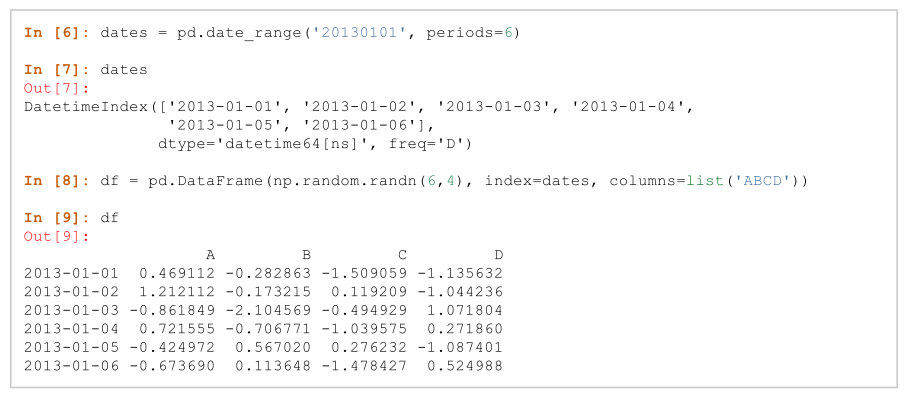
\includegraphics[width=\linewidth,keepaspectratio]{df1}
\end{center}
\end{frame}


%%%%%%%%%%%%%%%%%%%%%%%%%%%%%%%%%%%%%%%%%%%%%%%%%%%%%%%%%%%
\begin{frame}[fragile]\frametitle{Creating Dataframes}
Creating a DataFrame by passing a dict of objects that can be converted to series-like.
\begin{center}
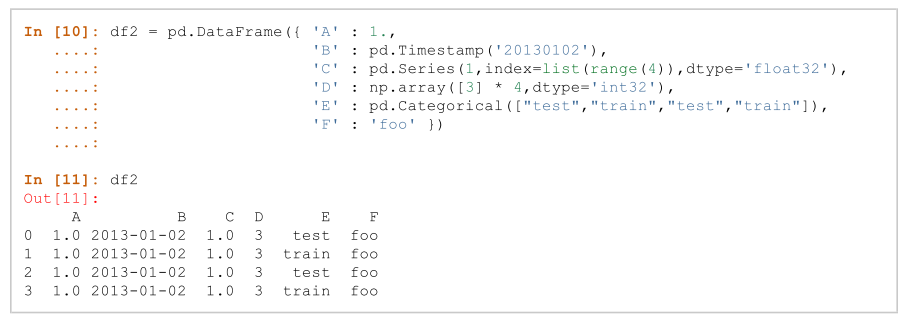
\includegraphics[width=\linewidth,keepaspectratio]{df2}
\end{center}
\end{frame}

%%%%%%%%%%%%%%%%%%%%%%%%%%%%%%%%%%%%%%%%%%%%%%%%%%%%%%%%%%%
\begin{frame}[fragile]\frametitle{Viewing Data}
See the top \& bottom row s of the frame
\begin{center}
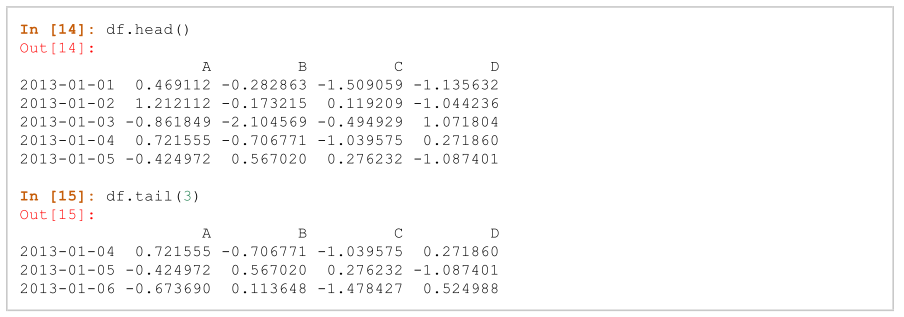
\includegraphics[width=\linewidth,keepaspectratio]{df3}
\end{center}
\end{frame}

%%%%%%%%%%%%%%%%%%%%%%%%%%%%%%%%%%%%%%%%%%%%%%%%%%%%%%%%%%%
\begin{frame}[fragile]\frametitle{Viewing Data}
Display the index, columns, and the underlying numpy data
\begin{center}
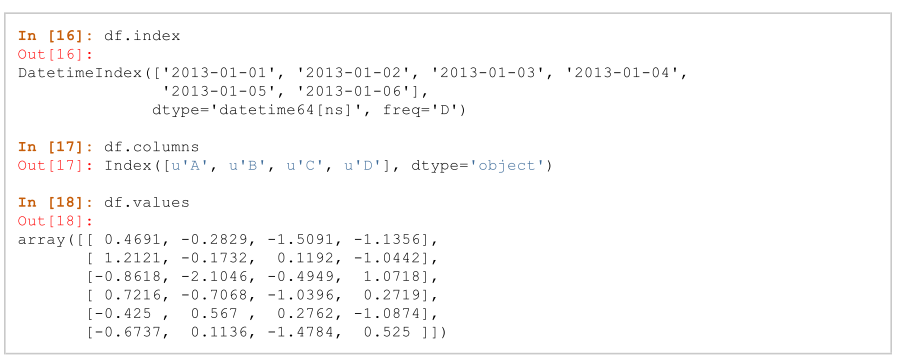
\includegraphics[width=\linewidth,keepaspectratio]{df4}
\end{center}
\end{frame}


%%%%%%%%%%%%%%%%%%%%%%%%%%%%%%%%%%%%%%%%%%%%%%%%%%%%%%%%%%%
\begin{frame}[fragile]\frametitle{Viewing Data}
Describe show s a quick statistic summary of your data
\begin{center}
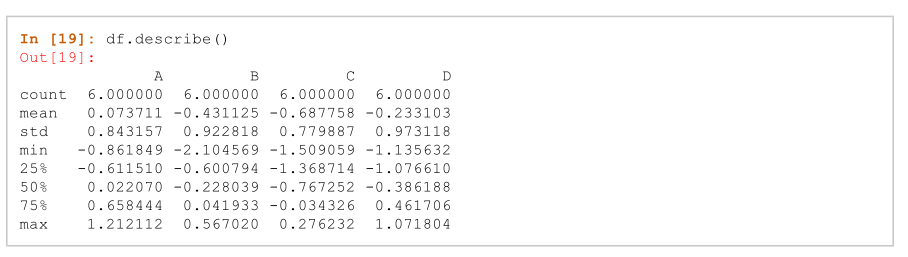
\includegraphics[width=\linewidth,keepaspectratio]{df5}
\end{center}
\end{frame}

%%%%%%%%%%%%%%%%%%%%%%%%%%%%%%%%%%%%%%%%%%%%%%%%%%%%%%%%%%%
\begin{frame}[fragile]\frametitle{Viewing Data}
Sorting by an axis
\begin{center}
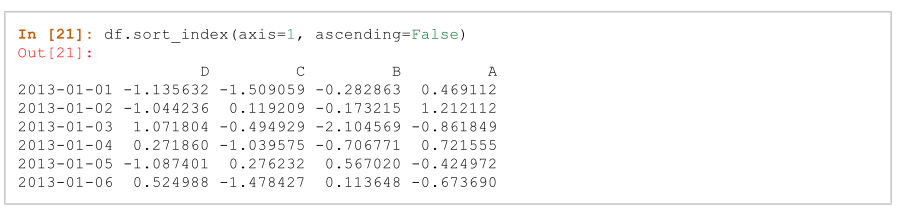
\includegraphics[width=\linewidth,keepaspectratio]{df6}
\end{center}
Sorting by values
\begin{center}
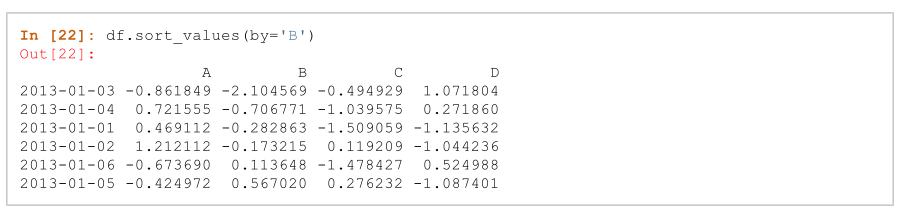
\includegraphics[width=\linewidth,keepaspectratio]{df7}
\end{center}
\end{frame}

%%%%%%%%%%%%%%%%%%%%%%%%%%%%%%%%%%%%%%%%%%%%%%%%%%%%%%%%%%%
\begin{frame}[fragile]\frametitle{Selection of  Data}
Selecting a single column, which yields a Series, equivalent to df.A
\begin{center}
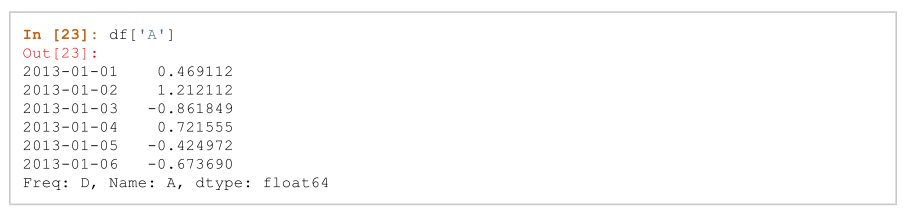
\includegraphics[width=\linewidth,keepaspectratio]{df8}
\end{center}

\end{frame}

%%%%%%%%%%%%%%%%%%%%%%%%%%%%%%%%%%%%%%%%%%%%%%%%%%%%%%%%%%%
\begin{frame}[fragile]\frametitle{Selection of  Data}
Selecting via [], which slices the row s.
\begin{center}
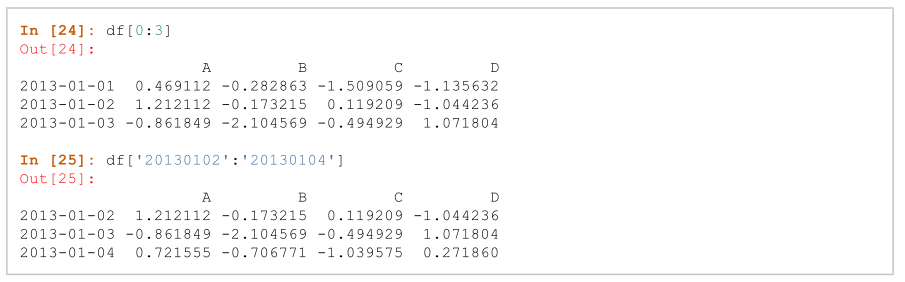
\includegraphics[width=\linewidth,keepaspectratio]{df9}
\end{center}
\end{frame}

%%%%%%%%%%%%%%%%%%%%%%%%%%%%%%%%%%%%%%%%%%%%%%%%%%%%%%%%%%%
\begin{frame}[fragile]\frametitle{Selection of  Data}
Selecting on a multi-axis by label
\begin{center}
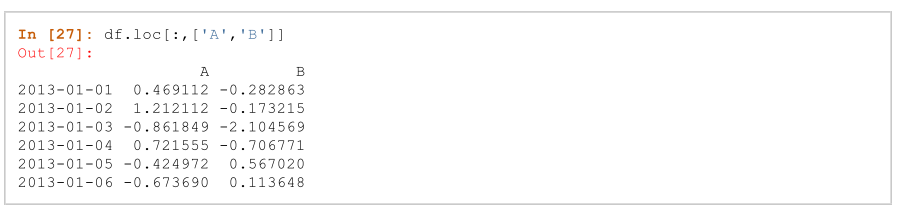
\includegraphics[width=\linewidth,keepaspectratio]{df10}
\end{center}
\end{frame}

%%%%%%%%%%%%%%%%%%%%%%%%%%%%%%%%%%%%%%%%%%%%%%%%%%%%%%%%%%%
\begin{frame}[fragile]\frametitle{Selection of  Data}
By integer slices, acting similar to numpy/python
\begin{center}
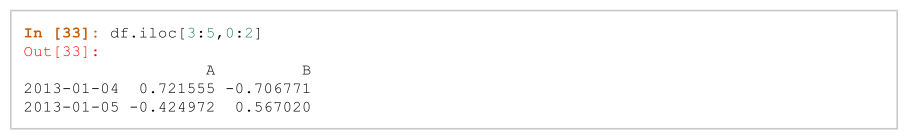
\includegraphics[width=\linewidth,keepaspectratio]{df11}
\end{center}
By lists of integer position locations, similar to the numpy/python style
\begin{center}
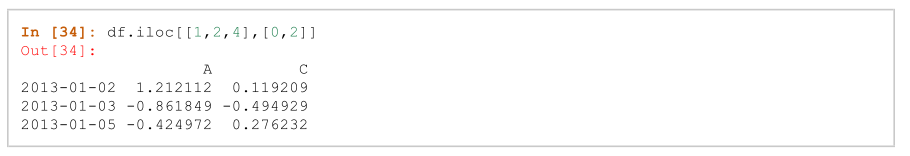
\includegraphics[width=\linewidth,keepaspectratio]{df12}
\end{center}
\end{frame}

%%%%%%%%%%%%%%%%%%%%%%%%%%%%%%%%%%%%%%%%%%%%%%%%%%%%%%%%%%%
\begin{frame}[fragile]\frametitle{ Boolean Indexing}
Using a single column's values to select data.
\begin{center}
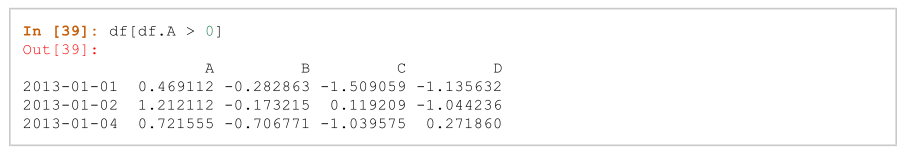
\includegraphics[width=\linewidth,keepaspectratio]{df13}
\end{center}
\end{frame}

%%%%%%%%%%%%%%%%%%%%%%%%%%%%%%%%%%%%%%%%%%%%%%%%%%%%%%%%%%%
\begin{frame}[fragile]\frametitle{ Missing Data}
To drop any row s that have missing data.
\begin{center}
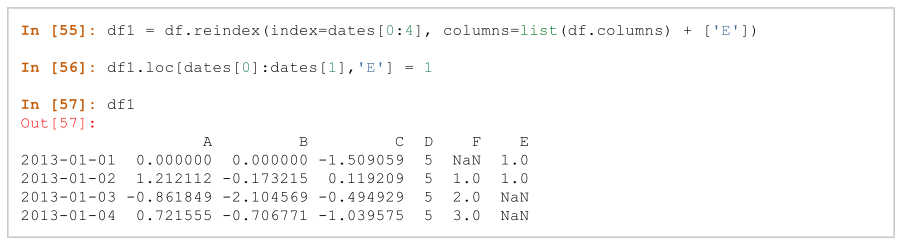
\includegraphics[width=\linewidth,keepaspectratio]{df14}
\end{center}
Filling missing data
\begin{center}
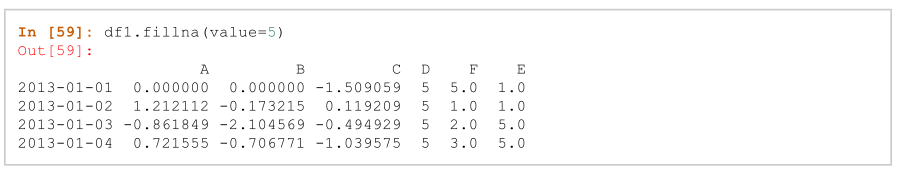
\includegraphics[width=\linewidth,keepaspectratio]{df15}
\end{center}
\end{frame}

%%%%%%%%%%%%%%%%%%%%%%%%%%%%%%%%%%%%%%%%%%%%%%%%%%%%%%%%%%%
\begin{frame}[fragile]\frametitle{ Stats}
Operations in general exclude missing data.
\begin{center}
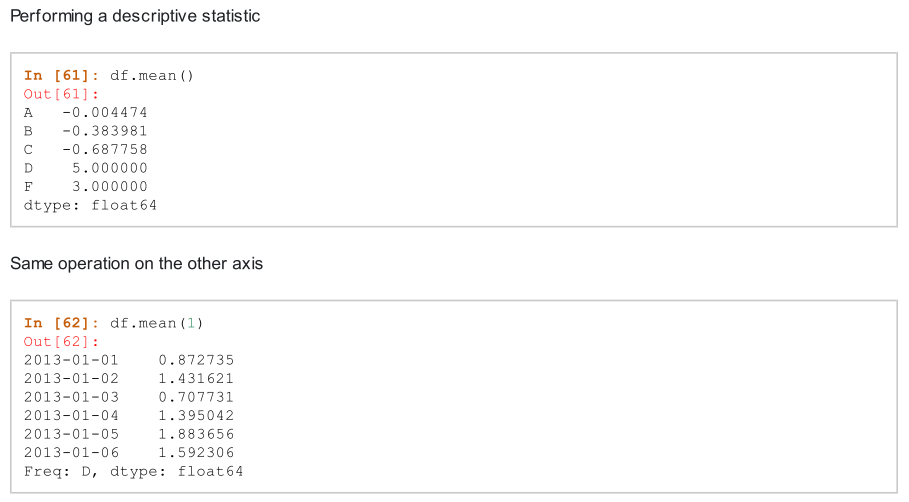
\includegraphics[width=\linewidth,keepaspectratio]{df16}
\end{center}
\end{frame}

%%%%%%%%%%%%%%%%%%%%%%%%%%%%%%%%%%%%%%%%%%%%%%%%%%%%%%%%%%%
\begin{frame}[fragile]\frametitle{ Apply}
Applying functions to the data
\begin{center}
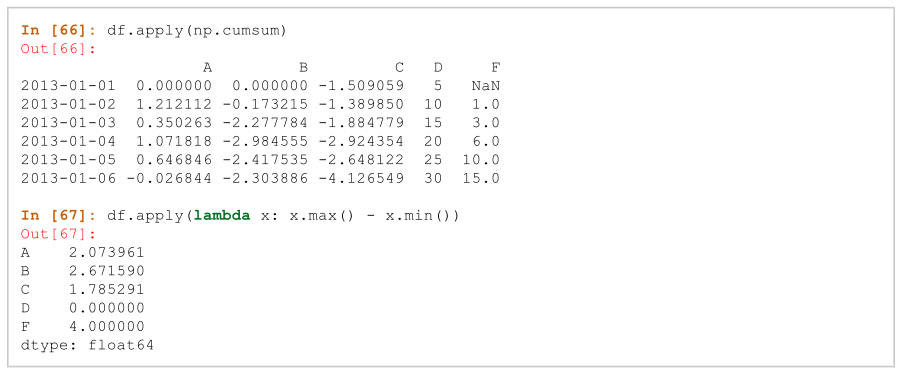
\includegraphics[width=\linewidth,keepaspectratio]{df17}
\end{center}
\end{frame}